\documentclass[12pt]{article}

%\usepackage{a4wide}
\usepackage{amsfonts}
%\usepackage{amssymb}
\usepackage{hyperref}
\usepackage{graphicx}
\usepackage{color}
\usepackage{macros}

%\bibliographystyle{plain}

\begin{document}

\title{Local Code Observables}
\vspace{1cm}
\date{\Large \today}
\author{\gene Development Team}

\maketitle

\vspace{2cm}
\begin{center}
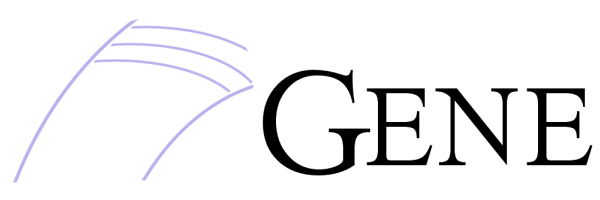
\includegraphics[width=\textwidth]{gene_logo2.png}
\end{center}

\thispagestyle{empty}

\newpage

\section{Basics}
\label{sec:basics}
For comparison with experimental results, all observable should ideally be given as functions of the particale coordinates. However, as \gene evolves the distribution function in gyrocenter coordinates, a mapping from gyrocenter to particle space is required.\\
\\
In Lie-formulation, a pull-back operator $T^*$ is employed for this reason which is given by
\bea
f^{(pc)}_{1\spec} & = T^* f^{(gc)}_{1\spec} \nn \\
& = f_{1\spec}^{(gc)} + \left[q_\spec \left(\avg{{\phi}_1}^{(gc)} -\phi_1^{(pc)} \right) + \mu \bar{B}_{1\|}^{(gc)} \right]\frac{F_{0\spec}}{T_{0\spec}} \\
& \equiv h_{1\spec}^{(gc)} - q_\spec \phi_1^{(pc)} \frac{F_{0\spec}}{T_{0\spec}} 
\label{eq:pc2gc}
\eea
if a Maxwellian background distribution is taken into account. In the local approximation, both gyroaveraged potentials/fields can be easily expressed by multiplications with Bessel functions, $\avg{{\phi}_1}^{(gc)} = J_0(k_\perp\rho) {\phi}_1^{(gc)}$ and $\bar{B}_{1\|}^{(gc)} = I_1(k_\perp\rho) B_{1\|}^{(gc)}$. Note that $I_1$ does {\bf !not!} denote the modified Bessel function but $I_1(x)=2 J_1(x) / x$.\\
\\
%Alternatively, a ``Frieman-Chen`` representation can be used (compare e.g.~ref.~\cite{Schekochihin09}, Eq.~124),
% \bea
% f^{\rm part. coord.}_{1\spec} & = -q \phi_1 \frac{F_{0\spec}}{T_{0\spec}} + h_{1\spec} \nn \\
% %& = -q_\spec \phi_1 \frac{F_{0\spec}}{T_{0\spec}} + \left(f_{1\spec} + 
% %q_\spec \frac{F_{0\spec}}{T_{0\spec}} 
% %\avg{\phi_1 - \frac{1}{c}\mvec{v}_\perp\cdot\mvec{A}_\perp} \right)
% & = -q_\spec \phi_1 \frac{F_{0\spec}}{T_{0\spec}} + \left(f_{1\spec} + 
% \sum_{\mvec{k}_\perp} \e^{\I \mvec{k}_\perp\cdot \mvec{R}_\spec} q_\spec \frac{F_{0\spec}}{T_{0\spec}} 
% \left(J_0(k_\perp\rho_\spec) \phi_1 + \frac{\mu}{q_\spec}I_1(k_\perp\rho_\spec)B_{1\|}\right) \right)
% \eea
Matter or energy are mainly advected by the drift velocity $\mvec{v}_D$ which is mostly determined by the generalized 
$\mvec{E}\times\mvec{B}$ velocity 
\bea
\mvec{v}_{\mpt} = \frac{c}{B_0^2}\mvec{B}_0\times\nabla\mpt_1
\eea
where 
$\mpt_1 = \phi_1-\frac{v_\|}{c}A_{1\|}-\frac{1}{c}\mvec{v}_\perp\cdot\mvec{A}_{1\perp}$
denotes the scalar potential in the gyrocenter moving frame which in general depends on the gyroangle(!).\\
Often, only the contravariant component in the radial direction 
is of interest which can be written as
\bea
v_\mpt^x & = \mvec{v}_{\mpt}\cdot\nabla x/\abs{\nabla x} \nn \\
& = -\frac{c}{\tilde\cofac}\frac{g^{11}g^{2i}-g^{1i}g^{21}}{\gamma_1}\partial_i \mpt_1 
%\nn \\
%& 
\approx 
-\frac{c}{\tilde\cofac}\,\partial_y \mpt_1
\eea
where $\tilde\cofac = \cofac \sqrt{g^{11}}$.\\
{\em Note:} Up to rev.~3189, only $\nabla x$ has been used for the projection in the $x$ direction.

\newpage
\section{Moments}

\subsection{Definition}
Many observables are based on velocity space moments of the particle coordinate distribution function
\bea
M_{ab,\spec}(\mvec{x}) = \int\!\!\D^3v\,\,v_\|^a v_\perp^b f^{(pc)} 
\eea
\\
Gyrocenter representation using the following Jacobian 
\bea
\D^3v = \int\D^3 X \D v_\| \D\mu \D\theta \,\, \delta(\mvec{X}+\mvec{r}-\mvec{x}) \frac{B_{0\|}^*}{m_\spec} 
\eea
gives
\bea
M_{ab,\spec}(\mvec{x}) = & \int\!\!\D^3 X \D v_\| \D\mu \D\theta \,\, \delta(\mvec{X}+\mvec{r}-\mvec{x}) \frac{B_{0\|}^*}{m_\spec} 
v_\|^a v_\perp^b \left\{ h_{1\spec}(\mvec{X}) - \frac{q_\spec F_{0\spec}}{T_{0\spec}}\phi_{1}(\mvec{x}) \right\} \nn \\
= & \int\!\!\D v_\| \D\mu \D\theta \,\, \frac{B_{0\|}^*}{m_\spec} 
v_\|^a v_\perp^b \left\{ h_{1\spec}(\mvec{x}-\mvec{r}) - \frac{q_\spec F_{0\spec}}{T_{0\spec}}\phi_{1}(\mvec{x}) \right\}
\eea

Assuming a Maxwellian equilibrium distribution function yields after some calculus (see, for instance, Ref.~\cite{GoerlerPhD09})
\bea
M_{ab,\spec}(\mvec{x}) = & \pi\left(\frac{2B_0}{m_\spec}\right)^{b/2+1}\iint \frac{B_{0\|}^*}{B_0} J_0 f_{1\spec} v_\|^a \mu^{b/2}  \D v_\| \D\mu -\frac{n_{0\spec} B_0}{T_{0\spec}^2} v_{T_\spec}^{a} \left(\frac{2B_0}{m_\spec}\right)^{b/2} \nn \\
& \cdot\left[\Upsilon(a) + \frac{8\pi T_{0\spec}}{B_0^2} \frac{j_{0\|}}{q_\spec v_{T\spec}} \Upsilon(a+1)\right] \left\{
\left(\frac{T_{0\spec}}{B_0}\right)^{b/2+1}\left(b/2\right)!\, q_\spec\phi_1(\mvec{x}) \right. 
\nn \\
& \left. -\int \left(q_\spec J_0^2 \phi_1+\mu J_0 I_1 {B}_{1\|}\right)
\e^{-\frac{\mu B_0}{T_{0\spec}}} \mu^{b/2}  \D\mu \right\} \label{eq:vsp-moment}
\eea
with the abbreviation
\bea
\Upsilon(a)=\frac{1}{\sqrt{\pi}}\int_{-\infty}^{\infty}x^a {\rm e}^{-x^2} dx =
\begin{cases} 
0, & a \mbox{ odd} \\ 
1, & a=0 \\
\frac{1\cdot3\cdots(a-1)}{\sqrt{2}^a} & a \mbox{ even}
\end{cases}
\eea
for the $v_\|$ integral. The normalized version is
\bea
\hat{M}_{ab,\spec}(\mvec{x}) = & M_{ab,\spec}(\mvec{x}) / \left[n_\rf c_\rf^{a+b}\roL \hat{n}_{0\spec}(\xp) \hat{v}_{T\spec}^{a+b}(\xp)\right] \nn \\
= & \pi\hat{B}_0^{b/2}
\iint \hat{B}_{0\|}^* J_0 \hat{f}_{1\spec} \hat{v}_\|^a \hat{\mu}^{b/2}  \D \hat{v}_\| \D\hat{\mu} \nn \\
& -\frac{\hat{n}_{p\spec}}{\hat{T}_{0\spec}}\hat{T}_{p\spec}^{(a+b)/2} 
\left[\Upsilon(a) + \beta_\rf \frac{\hat{T}_{0\spec}}{\hat{B}_0^2} \frac{\hat{j}_{0\|}}{\hat{q} \hat{v}_{T\spec}} \Upsilon(a+1)\right]
 \Bigg( (b/2)!\, \hat{q}_\spec\hat{\phi}_1(\mvec{x}) \Bigg. \nn \\
& \Bigg. - \left(\frac{\hat{B}_0}{\hat{T}_{p\spec}}\right)^{\frac{b}{2}+1}\!\!\int \left(\hat{q}_\spec J_0^2 \hat{\phi}_1
+\hat{T}_{0\spec}(\xp)\hat{\mu} J_0 I_1 \hat{\bar{B}}_{1\|}\right)
\e^{-\frac{\hat{\mu} \hat{B}_0}{\hat{T}_{p\spec}}} \hat{\mu}^{b/2}  \D\hat{\mu} \Bigg). \label{eq:vsp-moment-norm}
\eea

\subsection{Examples}
A few moments being used in the following 
({\bf neglecting equilibrium currents which can be of the same order!; 
however, the field equations would need to be adapted first})
% non-normalized version
% \bea
% M_{00,\spec}(\mvec{x}) = & \frac{2\pi B_0}{m_\spec} \iint J_0 f_{1\spec} \D v_\| \D\mu  \nn \\
% & -{n_{0\spec}}\left\{(1-\Gamma_0) \frac{q_\spec\phi_1}{T_{0\spec}} - 
% \left(\Gamma_0(b_\spec)-\Gamma_1(b_\spec)\right) \frac{{B}_{1\|}}{B_0} \right\} \\[1ex]
% %
% M_{10,\spec}(\mvec{x}) = &\frac{2\pi B_0}{m_\spec}\iint J_0 f_{1\spec} v_\| \D v_\| \D\mu \\[1ex]
% %
% M_{20,\spec}(\mvec{x}) 
% = & \frac{2\pi B_0}{m_\spec} \iint J_0 f_{1\spec} v_\|^2 \D v_\| \D\mu \nn \\
% & -\frac{1}{2} {n_{0\spec}} v_{T_\spec}^{2} \left\{ (1-\Gamma_0(b_\spec)) \frac{q_\spec\phi_1}{T_{0\spec}}
% -\Delta(b_\spec) \frac{B_{1\|}}{B_0}\right\} \\[1ex]
% %
% M_{02,\spec}(\mvec{x}) 
% % % = & \pi\left(\frac{2B_0}{m_\spec}\right)^2 \iint J_0 f_{1\spec} \mu \D v_\| \D\mu 
% % % -\frac{n_{0\spec} B_0}{T_{0\spec}^2} \left(\frac{2B_0}{m_\spec}\right) \nn \\
% % % & \cdot \left\{\left(\frac{T_{0\spec}}{B_0}\right)^2 q_\spec\phi_1(\mvec{x}) \right. 
% % % \nn \\
% % % & \left. -\int \left(q_\spec J_0^2 \phi_1+\mu J_0 I_1 {B}_{1\|}\right)
% % % \e^{-\frac{\mu B_0}{T_{0\spec}}} \mu  \D\mu \right\} \nn \\
% = & \pi\left(\frac{2B_0}{m_\spec}\right)^2 \iint J_0 f_{1\spec} \mu \D v_\| \D\mu \nn \\
% & -n_{0\spec} v_{T\spec}^2 \left\{\left[1 - \Gamma_0(b_\spec)+b_\spec \Delta(b_\spec)\right] \frac{q_\spec\phi_1}{T_{0\spec}} \right. \nn \\
% & \left. \hspace{5em} -\left[ \Gamma_0(b_\spec) + (1-2 b_\spec) \Delta(b_\spec) \right] \frac{{B}_{1\|}}{B_0} \right\} 
% %
% \eea

\bea
\hat{M}_{00,\spec}(\mvec{x}) = & \pi\hat{B}_0
\iint J_0 \hat{f}_{1\spec} \D \hat{v}_\| \D\hat{\mu} \nn \\
& -\left\{(1-\Gamma_0) \frac{\hat{q}_\spec\hat{\phi}_1}{\hat{T}_{0\spec}} - 
\Delta(b_\spec) \frac{\hat{B}_{1\|}}{\hat{B}_0} \right\} \\[1ex]
%
\hat{M}_{10,\spec}(\mvec{x}) = & \pi\hat{B}_0 \iint J_0 \hat{f}_{1\spec} \hat{v}_\| \D \hat{v}_\| \D\hat{\mu} \\
%
\hat{M}_{20,\spec}(\mvec{x}) 
= & \pi\hat{B}_0 \iint J_0 \hat{f}_{1\spec} \hat{v}_\|^2 \D \hat{v}_\| \D\hat{\mu} \nn \\
& -\frac{1}{2} \left\{ (1-\Gamma_0(b_\spec)) \frac{\hat{q}_\spec\phi_1}{\hat{T}_{0\spec}}
-\Delta(b_\spec) \frac{\hat{B}_{1\|}}{\hat{B}_0}\right\} \\[1ex]
%
\hat{M}_{02,\spec}(\mvec{x}) = & \pi\hat{B}_0^2
\iint J_0 \hat{f}_{1\spec} \hat{\mu} \D \hat{v}_\| \D\hat{\mu} \nn \\
& - \left\{\left[1 - \Gamma_0(b_\spec)+b_\spec \Delta(b_\spec)\right] \frac{\hat{q}_\spec \hat{\phi}_1}{\hat{T}_{0\spec}} 
- \left[ \Gamma_0(b_\spec) + (1-2 b_\spec) \Delta(b_\spec) \right]\frac{\hat{B}_{1\|}}{\hat{B}_0}\right\}
%
\eea
Here, $\Gamma_n = \hat{I}_n(x) {\rm e}^{-\abs{x}}$ with the modified Bessel function $\hat{I}_n(x)$ (not to be confused with $I_n(x)$).

\subsection{$I_1$ velocity space moment}

Furthermore, a velocity space moment including a $\mu I_1$ operation on $h_{1\spec}$ is defined:
\bea
N_{ab,\spec} & = \pi \left(\frac{2 B_0}{m_\spec}\right)^{b/2+1}
 \int\!\!\D v_\| \D\mu \,\, v_\|^a \mu^{b/2} \mu B_0 I_1 h_{1\spec,\mvec{k}} \nn \\
& = \pi \left(\frac{2 B_0}{m_\spec}\right)^{b/2+1}
\int\!\!\D v_\| \D\mu \,\, v_\|^a \mu^{b/2} \mu B_0 I_1 
\left[f_{1\spec,\mvec{k}} + \left(q_\spec J_0 \phi_1 + \mu I_1 B_{\|1}\right)\frac{F_{0\spec}}{T_{0\spec}}\right]
\eea

Normalized version
\bea
\hat{N}_{ab,\spec} = & N_{ab,\spec} / \left[p_\rf c_\rf^{a+b} \roL \hat{p}_{0\spec}(\xp) \hat{v}^{a+b}_{T\spec}(\xp)\right]  \nn \\
 = &  \left\{ \pi \hat{B}_0^{b/2+2}
\int\!\!\D \hat{v}_\| \D\hat{\mu} \,\, \hat{v}_\|^a \hat{\mu}^{b/2} \hat{\mu} I_1 
\left[\hat{f}_{1\spec,\mvec{k}} + \left(\hat{q}_\spec J_0 \hat{\phi}_1 + \hat{T}_{0\spec}(\xp) 
\hat{\mu} I_1 \hat{B}_{\|1}\right)\frac{\hat{F}_{0\spec}}{\hat{T}_{0\spec}}\right] \right\}
\eea


\subsubsection{Examples}
% non-normalized
% \bea
% N_{00,\spec} 
% = & \frac{2\pi B_0^2}{m_\spec} \int\!\!\D v_\| \D\mu \,\, \mu I_1 f_{1\spec,\mvec{k}} \nn \\
% & + p_{0\spec} \Delta(b_\spec) 
% \left(\frac{q_\spec \phi_1}{T_{0\spec}}  + 2 \frac{B_{\|1}}{B_0}\right) \\[1ex]
% %
% N_{20,\spec} 
% = & \frac{2\pi B_0^2}{m_\spec} \int\!\!\D v_\| \D\mu \,\, v_\|^2 \mu I_1 f_{1\spec,\mvec{k}} \nn \\
% & + \frac{1}{2} v_{T\spec}^2 p_{0\spec}\Delta(b_\spec) 
% \left[\frac{q_\spec \phi_1}{T_{0\spec}} + 2 \frac{B_{\|1}}{B_0}\right] \\[1ex]
% %
% N_{02,\spec} 
% = & \frac{4\pi B_0^3}{m_\spec^2} \int\!\!\D v_\| \D\mu \,\, \mu^2 I_1 f_{1\spec,\mvec{k}} \nn \\
% & + v_{T\spec}^2 p_{0\spec}
% \left( \left[ \Gamma_0(b_\spec) + (1-2 b_\spec) \Delta(b_\spec) \right] \frac{q_\spec \phi_1}{T_{0\spec}} \right. \nn \\
% & \phantom{+ \frac{n_{0\spec} T_{0\spec}^2}{B_0^2}} \left. +  2 \left[\Gamma_0(b_\spec) + 2 (1-b_\spec) \Delta(b_\spec)\right] \frac{B_{\|1}}{B_0}\right)
% \eea

\bea
\hat{N}_{00,\spec} 
= & \pi \hat{B}_0^2 \int\!\!\D \hat{v}_\| \D\hat{\mu} \,\, \hat{\mu} I_1 \hat{f}_1 \nn \\
& + \Delta(b_\spec)
\left(\frac{\hat{q}_\spec \hat{\phi}_1}{\hat{T}_{0\spec}}  + 2 \frac{\hat{B}_{\|1}}{\hat{B}_0}\right) \\[1ex]
%
\hat{N}_{20,\spec} 
= & \pi \hat{B}_0^2 \int\!\!\D \hat{v}_\| \D\hat{\mu} \,\, \hat{v}_\|^2 \hat{\mu} I_1 \hat{f}_{1\spec} \nn \\
& + \frac{\Delta(b_\spec) }{2}
\left[\frac{\hat{q}_\spec \hat{\phi}_1}{\hat{T}_{0\spec}} + 2 \frac{\hat{B}_{\|1}}{\hat{B}_0}\right] \\[1ex]
%
\hat{N}_{02,\spec} 
= & \pi \hat{B}_0^3 \int\!\!\D \hat{v}_\| \D\hat{\mu} \,\, \hat{\mu}^2 I_1 \hat{f}_{1\spec} \nn \\
& + \left( \left[ \Gamma_0(b_\spec) + (1-2 b_\spec) \Delta(b_\spec) \right] \frac{\hat{q}_\spec \hat{\phi}_1}{\hat{T}_{0\spec}} \right. \nn \\
& \phantom{+ \frac{n_{0\spec} T_{0\spec}^2}{B_0^2}} \left. +  2 \left[\Gamma_0(b_\spec) + 2 (1-b_\spec) \Delta(b_\spec)\right] \frac{\hat{B}_{\|1}}{\hat{B}_0}\right)
\eea

\subsection{Application}
Typically, the following moments (or combinations of moments) are evaluated in \gene (assuming a Local Maxwellian equilibrium distribution function and thus $u_{0\|} = 0$)
\bea
n_{1\spec}(\mvec{x}) & = \int\!\!\D^3v\,\, f^{(pc)} = M_{00,\spec}(\mvec{x}) \\
u_{1\|\spec}(\mvec{x}) & = \frac{1}{n_{0\spec}} \int\!\!\D^3v\,\,v_\| f^{(pc)} = \frac{1}{n_{0\spec}} M_{10,\spec}(\mvec{x}) \\
T_{1\|\spec}(\mvec{x}) & = \frac{m_\spec}{n_{0\spec}} \int\!\!\D^3v\,\,(v_\|-u_{1\|,\spec})^2 f^{(pc)} - T_{0\spec} \frac{n_{1\spec}}{n_{0\spec}} \nn \\
& \approx \frac{2 M_{20,\spec}(\mvec{x}) - T_{0\spec} M_{00,\spec}(\mvec{x})}{n_{0\spec}} \\
T_{1\perp\spec}(\mvec{x}) & = \frac{m_\spec}{2n_{0\spec}} \int\!\!\D^3v\,\,v_\perp^2 f^{(pc)} - T_{0\spec} \frac{n_{1\spec}}{n_{0\spec}} \nn \\ & = \frac{M_{02,\spec}(\mvec{x}) - T_{0\spec} M_{00,\spec}(\mvec{x})}{n_{0\spec}}
\eea
such that the total temperature fluctuation is given by $T_{1} = (T_{1\|} + 2 T_{1\perp})/3$.\\
Furthermore, the parallel and perpendicular heat current densities (here just electrostatic)
\bea
q_{\|}(\mvec{x}) & = \frac{m_\spec}{2} \int\!\!\D^3v\,\,\left(v_\|-u_\|\right)^3 f^{(pc)} \nn \\
q_{1\|}(\mvec{x}) & \approx \frac{m_\spec}{2} M_{30,\spec} (\mvec{x}) - \frac{3}{2} p_{0\spec} u_{1\|}(\mvec{x}) \\
q_{1\perp}(\mvec{x}) & = \frac{m_\spec}{2} \int\!\!\D^3v\,\,v_\perp^2 \left(v_\|-u_\|\right) f^{(pc)} \nn \\
q_{\perp}(\mvec{x}) & \approx \frac{m_\spec}{2} M_{12,\spec} (\mvec{x}) - p_{0\spec} u_{1\|}(\mvec{x})
\eea
are evaluated indirectly, as \gene writes out $M_{30,\spec} (\mvec{x})$ and $M_{12,\spec} (\mvec{x})$.\\
TODO: Add electromagnetic contributions, similarly to Sec.~\ref{subsec:heatflux} !!!

\newpage
\section{Fluxes}

Fluxes appear to be somewhat more complicated as the multiplication with the drift velocity introduces an additional gyroangle dependence via  the $\mvec{v}_\perp\cdot\mvec{A}_{1\perp}$ term.

\subsection{Particle flux}

Basic definition
\bea
\mvec{\Gamma}_\spec(\mvec{x}) = \int\!\!\D^3v\,\, f^{(pc)}\,\, \mvec{v}_D \, 
\eea
\\
Gyrocenter representation neglecting equilibrium currents
\bea
\mvec{\Gamma}_\spec(\mvec{x}) = & \int\!\!\D^3 X \D v_\| \D\mu \D\theta \,\, \delta(\mvec{X}+\mvec{r}-\mvec{x}) \frac{B_0}{m_\spec} 
\left\{ h_{1\spec}(\mvec{X}) - \frac{q_\spec F_{0\spec}}{T_{0\spec}}\phi_{1}(\mvec{x}) \right\} \mvec{v}_{D}^{\phantom{pc}}(\mvec{x}) \nn \\
= & \int\!\!\D v_\| \D\mu \D\theta \,\, \frac{B_0}{m_\spec} 
\left\{ h_{1\spec}(\mvec{x}-\mvec{r}) - \frac{q_\spec F_{0\spec}}{T_{0\spec}}\phi_{1}(\mvec{x}) \right\} \mvec{v}_{D}^{\phantom{pc}}(\mvec{x})
\eea
%with $h_{1\spec}(\mvec{X}) = f_{1\spec}(\mvec{X}) + \left[q_\spec \avg{{\phi}_{1}}(\mvec{X}) + \mu \bar{B}_{1\|}(\mvec{X})\right]\frac{F_{0\spec}}{T_{0\spec}}$.\\
\\
Fourier representation
% \bea
% \mvec{\Gamma}_\spec = & \frac{B_0}{m_\spec} \sum_{\mvec{k},\mvec{k}^\prime} \e^{\I (\mvec{k}+\mvec{k}^\prime)\mvec{x}}
% \int\!\!\D v_\| \D\mu \D\theta \,\, \left\{ f_{1\spec,\mvec{k}} 
% \e^{-\I \mvec{k}\mvec{r}} - \frac{q_\spec F_{0\spec}}{T_{0\spec}}\phi_{1,\mvec{k}} + \right. \nn \\
% & \left. \hspace{1cm} \left[q_\spec J_0(k_\perp\rho){\phi}_{1,\mvec{k}}\e^{-\I \mvec{k}\mvec{r}} + \mu I_1(k_\perp\rho) B_{1\|,\mvec{k}}\e^{-\I \mvec{k}\mvec{r}} \right] \frac{F_{0\spec}}{T_{0\spec}} \right\} \nn \\ %\mvec{v}_{D,\mvec{k}^\prime}^{\phantom{pc}}
% & \hspace{1cm} \frac{c}{B_0^2}\mvec{B}_0\times (\I \mvec{k}^\prime) \left[\phi_{1,\mvec{k}^\prime}-\frac{v_\|}{c}A_{1\|,\mvec{k}^\prime}-\frac{1}{c}\mvec{v}_\perp\cdot\mvec{A}_{1\perp,\mvec{k}^\prime}\right] 
% \eea
\bea
\mvec{\Gamma}_\spec = & \frac{B_0}{m_\spec} \sum_{\mvec{k},\mvec{k}^\prime} \e^{\I (\mvec{k}+\mvec{k}^\prime)\mvec{x}}
\int\!\!\D v_\| \D\mu \D\theta \,\, \left\{ h_{1\spec,\mvec{k}} 
\e^{-\I \mvec{k}\mvec{r}} - \frac{q_\spec F_{0\spec}}{T_{0\spec}}\phi_{1,\mvec{k}} \right\} \nn \\ %\mvec{v}_{D,\mvec{k}^\prime}^{\phantom{pc}}
& \hspace{1cm} \frac{c}{B_0^2}\mvec{B}_0\times (\I \mvec{k}^\prime) \left[\phi_{1,\mvec{k}^\prime}-\frac{v_\|}{c}A_{1\|,\mvec{k}^\prime}-\frac{1}{c}\mvec{v}_\perp\cdot\mvec{A}_{1\perp,\mvec{k}^\prime}\right] 
\eea
\\
Gyro-averaging integrals (see, e.g, Refs.~\cite{DannertPhD05}, pp.~125, \cite{MerzPhD08}, pp.~117, and \cite{JenkoHabildraft}, Eq.~(2.139))\\
%{\em TODO: recheck the sign of Eq.~\ref{eq:gyav_intIII}}
\bea
\avg{\e^{-\I \mvec{k}\mvec{r}}} & = J_0(k_\perp\rho) \\
\avg{\mvec{v}_\perp \mvec{A}_{1\perp,\mvec{k}^\prime}} & = 
0 \qquad (\textrm{note: } \mvec{A}_{1\perp,\mvec{k}^\prime} \neq \mvec{A}_{1\perp,\mvec{k}^\prime}(\theta)!!)  \\ %- \frac{c}{q_\spec} \mu I_1(k_\perp\rho) B_{1\|} \\
\avg{\e^{-\I \mvec{k}\mvec{r}} \mvec{v}_\perp \mvec{A}_{1\perp,\mvec{k}^\prime}} & = 
\frac{c}{q_\spec} \mu I_1(k_\perp\rho) (\uvec{b}\times (\I \mvec{k})) \mvec{A}_{1\perp,\mvec{k}^\prime} \label{eq:gyav_intIII} \\
& \rightarrow \frac{c}{q_\spec} \mu I_1(k_\perp\rho) B_{1\|,\mvec{k}} \qquad \textrm{if } \mvec{k}=\mvec{k}^\prime \textrm{ only} \nn
\eea
\\
Projection in the $x$-direction and $\theta$-integration
\bea
\Gamma^x_\spec = & - \frac{c}{\tilde\cofac} \frac{2\pi B_0}{m_\spec} \sum_{\mvec{k},\mvec{k}^\prime} \e^{\I (\mvec{k}+\mvec{k}^\prime)\mvec{x}}
\int\!\!\D v_\| \D\mu \,\, (\I k_y^\prime) \bigg\{ \bigg.\nn \\
& \hspace{1cm} h_{1\spec,\mvec{k}} \left[J_0 \phi_{1,\mvec{k}^\prime}-\frac{v_\|}{c} J_0 A_{1\|,\mvec{k}^\prime}
- \frac{1}{q_\spec} \mu I_1(k_\perp\rho) (\uvec{b}\times (\I \mvec{k})) \mvec{A}_{1\perp,\mvec{k}^\prime} \right]   \nn \\ 
& \hspace{1cm} \left. - \frac{q_\spec F_{0\spec}}{T_{0\spec}}\phi_{1,\mvec{k}}
\left[\phi_{1,\mvec{k}^\prime}-\frac{v_\|}{c}A_{1\|,\mvec{k}^\prime} \right]
\right\}
\eea
\\
Perpendicular average and employing 
$\avg{\e^{\I (\mvec{k}+\mvec{k}^\prime)\mvec{x}}}_{\perp} = \delta_{\mvec{k},-\mvec{k}^\prime}$ 
and $f^{\phantom{*}}_\mvec{k} = f^*_{-\mvec{k}}$
\bea
\avg{\Gamma^x_\spec}_{\perp} = & - \frac{c}{\tilde\cofac}\frac{2\pi B_0}{m_\spec} \sum_{\mvec{k}}
\int\!\!\D v_\| \D\mu \,\, (\I k_y) \bigg\{ \bigg.\nn \\
& \hspace{1cm} h^*_{1\spec,\mvec{k}} \left[J_0 \phi_{1,\mvec{k}}-\frac{v_\|}{c} J_0 A_{1\|,\mvec{k}}
+ \frac{1}{q_\spec} \mu I_1(k_\perp\rho) B_{1\|,\mvec{k}} \right] \nn \\
& \hspace{1cm} \left. - \frac{q_\spec F_{0\spec}}{T_{0\spec}}\phi^*_{1,\mvec{k}}
\left[\phi_{1,\mvec{k}}-\frac{v_\|}{c}A_{1\|,\mvec{k}} \right]
\right\}
\eea

Using 
\bea
n_{1\spec,\mvec{k}} = & \frac{2\pi B_0}{m_\spec} \int\!\!\D v_\| \D\mu \,\, \left[J_0 f_{1\spec,\mvec{k}} 
+ \left( q_\sigma (J_0^2 - 1) \phi_{1,\mvec{k}} + \mu J_0 I_1 B_{1\|,\mvec{k}} \right) \frac{F_{0\spec}}{T_{0\spec}}\right] \nn \\
= & \frac{2\pi B_0}{m_\spec} \int\!\!\D v_\| \D\mu \,\, \left[J_0 h_{1\spec,\mvec{k}} 
 - q_\sigma \phi_{1,\mvec{k}}  \frac{F_{0\spec}}{T_{0\spec}}\right] = M_{00\spec,\mvec{k}}, \\
%
j_{1\|\spec,\mvec{k}} = & q_\spec \frac{2\pi B_0}{m_\spec} \int\!\!\D v_\| \D\mu \,\, v_\| 
\left[
J_0 h_{1\spec,\mvec{k}} - q_\sigma \phi_{1,\mvec{k}}  \frac{F_{0\spec}}{T_{0\spec}}
\right] = M_{10\spec,\mvec{k}}, \\
%
p_{1\perp\spec,\mvec{k}} \equiv & \frac{2\pi B_0}{m_\spec} \int\!\!\D v_\| \D\mu \,\, \mu B_0 I_1 h_{1\spec,\mvec{k}} = N_{00\spec,\mvec{k}}, \label{eq:pdef}
\eea
allows for the volume averaged (radial) particle transport to be rewritten as
\bea
\avg{\Gamma^x_\spec}_\perp
= & -\frac{c}{\tilde\cofac} \sum_{\mvec{k}} (\I k_y) \left[ n^*_{1\spec,\mvec{k}} \phi_{1,\mvec{k}} - \frac{1}{q_\spec c} j^*_{1\|\spec,\mvec{k}} A_{1\|,\mvec{k}} + \frac{1}{q_\spec} \frac{p^*_{1\perp\spec,\mvec{k}}}{B_0} B_{1\|,\mvec{k}} \right]
\eea



\subsubsection{Check for ambipolarity}

Field equations
\bea
\nabla_\perp^2 \phi_1 = & -4\pi \sum_\spec q_\spec n_{1\spec} \\
\nabla_\perp^2 A_{1\|} = & - \frac{4\pi}{c} \sum_\spec j_{1\|\spec} \\
B_{1\|} = & - 4\pi \sum_\spec \frac{p_{1\perp,\spec}}{B_0}
\eea

and thus

\bea
\sum_\spec q_\spec \avg{\Gamma^x_\spec}_\perp 
 = & -\frac{1}{4\pi}\frac{c}{\tilde\cofac} \sum_{\mvec{k}} \I k_y \left[ k_\perp^2 \abs{\phi_{1,\mvec{k}}}^2  - k_\perp^2 \abs{A_{1\|,\mvec{k}}}^2 - \abs{B_{1\|,\mvec{k}}}^2 \right] \nn \\
 = &\, 0 \qquad \textrm{q.e.d}
\eea

\subsubsection{Spectrum}

Following Ref.~\cite{Jenko99}, the definition
\bea
\avg{\Gamma^x_\spec}_\perp
= & \sum_{\mvec{k}} \frac{c}{\tilde\cofac} (-\I k_y) \left[ n^*_{1\spec,\mvec{k}} \phi_{1,\mvec{k}} - \frac{1}{q_\spec c} j^*_{1\|\spec,\mvec{k}} A_{1\|,\mvec{k}} + \frac{1}{q_\spec} \frac{p^*_{1\perp\spec,\mvec{k}}}{B_0} B_{1\|,\mvec{k}} \right] \nn \\
\equiv & \sum_{\mvec{k}} \Gamma^x_{\spec,\mvec{k}}
\eea
is employed for spectra of transport fluxes. Note that this choice captures the contributions from different wave numbers but cannot be applied for an inverse Fourier transform which would require the convolution of the fluctuating signals
\bea
\tilde{\Gamma}^x_{\spec,\mvec{k}} = &
- \frac{c}{\tilde\cofac} \frac{2\pi B_0}{m_\spec} \sum_{\mvec{k}^\prime}
\int\!\!\D v_\| \D\mu \,\, (\I k_y^\prime) \bigg\{ \bigg.\nn \\
& \hspace{1cm} h_{1\spec,\mvec{k}-\mvec{k}^\prime}  \left[J_0 \phi_{1,\mvec{k}^\prime}-\frac{v_\|}{c} J_0 A_{1\|,\mvec{k}^\prime}
- \frac{\mu I_1}{q_\spec}  (\uvec{b}\times (\I (\mvec{k}-\mvec{k}^\prime))) \mvec{A}_{1\perp,\mvec{k}^\prime} \right]   \nn \\ 
& \hspace{1cm} \left. - \frac{q_\spec F_{0\spec}}{T_{0\spec}}\phi_{1,\mvec{k}-\mvec{k}^\prime}
\left[\phi_{1,\mvec{k}^\prime}-\frac{v_\|}{c}A_{1\|,\mvec{k}^\prime} \right]
\right\}.
\eea

Furthermore, note that transport spectrum plots typically show only positive wavenumbers with negative ones being mapped. This way, the final results usually contains combinations like $2 \Re[ A^* B ]$.

\subsubsection{Implementation}

We might consider using $h_{1,\mvec{k}}$ in the diagnostics module in the future but currently moments are implemented with respect to $f_{1,\mvec{k}}$
\bea
\Gamma^x_{\spec,\mvec{k}}
= & - \frac{c}{\tilde\cofac}\frac{2\pi B_0}{m_\spec}
\int\!\!\D v_\| \D\mu \,\, (\I k_y) \bigg\{ \left(f^*_{1\spec,\mvec{k}} + 
\left[q_\spec J_0 \phi^*_{1,\mvec{k}} + \mu I_1 B^*_{1\|,\mvec{k}} \right]\frac{F_{0\spec}}{T_{0\spec}}\right) \bigg.\nn \\
& \hspace{1cm} \left[J_0 \phi_{1,\mvec{k}}-\frac{v_\|}{c} J_0 A_{1\|,\mvec{k}}
+ \frac{1}{q_\spec} \mu I_1(k_\perp\rho) B_{1\|,\mvec{k}} \right] \nn \\
& \hspace{1cm} \left. - \frac{q_\spec F_{0\spec}}{T_{0\spec}}\phi^*_{1,\mvec{k}}
\left[\phi_{1,\mvec{k}}-\frac{v_\|}{c}A_{1\|,\mvec{k}} \right]
\right\} 
\eea

%comment out
% % \bea
% % \Gamma^x_{\spec,\mvec{k}}
% % = & - \frac{c}{\tilde\cofac}\frac{2\pi B_0}{m_\spec}
% % \int\!\!\D v_\| \D\mu \,\, (\I k_y) \bigg\{ \bigg.\nn \\
% % & \hspace{1cm} f^*_{1\spec,\mvec{k}} \left[J_0 \phi_{1,\mvec{k}}-\frac{v_\|}{c} J_0 A_{1\|,\mvec{k}}
% % + \frac{1}{q_\spec} \mu I_1(k_\perp\rho) B_{1\|,\mvec{k}} \right] \nn \\
% % & \hspace{1cm} + \left[q_\spec J_0 \phi^*_{1,\mvec{k}} + \mu I_1 B^*_{1\|,\mvec{k}} \right]\frac{F_{0\spec}}{T_{0\spec}} 
% %  \left[J_0 \phi_{1,\mvec{k}} + \frac{1}{q_\spec} \mu I_1(k_\perp\rho) B_{1\|,\mvec{k}} \right] \nn \\
% % & \hspace{1cm} \left. - \frac{q_\spec F_{0\spec}}{T_{0\spec}}\abs{\phi_{1,\mvec{k}}}^2
% % \right\} 
% % \eea
% % 
% % 
% % \bea
% % \Gamma^x_{\spec,\mvec{k}}
% % = & - \frac{c}{\tilde\cofac}\frac{2\pi B_0}{m_\spec} (\I k_y)
% % \int\!\!\D v_\| \D\mu \,\, \bigg\{ 
% % f^*_{1\spec,\mvec{k}} \left[J_0 \phi_{1,\mvec{k}}-\frac{v_\|}{c} J_0 A_{1\|,\mvec{k}}
% % + \frac{\mu I_1}{q_\spec}  B_{1\|,\mvec{k}} \right] \bigg. \nn \\
% % & \left. + \left[
% % q_\spec (J_0^2-1) \abs{\phi_{1,\mvec{k}}}^2 + \mu J_0 I_1 2\Re[\phi^*_{1,\mvec{k}} B_{1\|,\mvec{k}}]
% % + \frac{1}{q_\spec} \mu^2 I_1^2 \abs{B_{1\|,\mvec{k}}}^2 
% % \right] \frac{F_{0\spec}}{T_{0\spec}}
% % \right\} 
% % \eea

Some rearranging and $(v_\|,\mu)$ integration (if possible)
%comment out:
% % \bea
% % \Gamma^x_{\spec,\mvec{k}}
% % = & - \frac{c}{\tilde\cofac}\frac{2\pi B_0}{m_\spec} (\I k_y)
% % \bigg\{ \int\!\!\D v_\| \D\mu \,\,  
% % f^*_{1\spec,\mvec{k}} \left[J_0 \phi_{1,\mvec{k}}-\frac{v_\|}{c} J_0 A_{1\|,\mvec{k}}
% % + \frac{\mu I_1}{q_\spec}  B_{1\|,\mvec{k}} \right] \bigg. \nn \\
% % &  + \frac{n_{0\spec}}{\pi v_{T\spec}^2 T_{0\spec}} \int\!\!\D\mu \,\, \left[
% % q_\spec (J_0^2-1) \abs{\phi_{1,\mvec{k}}}^2 + 2 \mu J_0 I_1 \Re[\phi^*_{1,\mvec{k}} B_{1\|,\mvec{k}}]
% %  \right. \nn \\
% % & \left. \left. + \frac{1}{q_\spec} \mu^2 I_1^2 \abs{B_{1\|,\mvec{k}}}^2 \right] \e^{- \mu B_0/T_{0\spec}}
% % \right\} 
% % \eea

% \bea
% \Gamma^x_{\spec,\mvec{k}}
% = & - \frac{c}{\tilde\cofac} (\I k_y)
% \bigg\{ \frac{2\pi B_0}{m_\spec} \int\!\!\D v_\| \D\mu \,\,  
% f^*_{1\spec,\mvec{k}} \left[J_0 \phi_{1,\mvec{k}}-\frac{v_\|}{c} J_0 A_{1\|,\mvec{k}}
% + \frac{\mu I_1}{q_\spec}  B_{1\|,\mvec{k}} \right] \bigg. \nn \\
% &  + \frac{n_{0\spec}}{T_{0\spec}} \left[
%  q_\spec (\Gamma_0-1) \abs{\phi_{1,\mvec{k}}}^2 
% + \frac{T_{0\spec}}{B_0} \left(\Gamma_0(b_\spec)-\Gamma_1(b_\spec)\right) 2 \Re[\phi^*_{1,\mvec{k}} B_{1\|,\mvec{k}}]
%  \right. \nn \\
% & \left. \left. + 2 \frac{T_{0\spec}^2}{B_0^2} \left(\Gamma_0(b_\spec)-\Gamma_1(b_\spec)\right) \frac{1}{q_\spec} \abs{B_{1\|,\mvec{k}}}^2 \right]
% \right\} 
% \eea

Split into electrostatic ($\mvec{A}=0$) and electromagnetic ({\em rest}) parts

% \bea
% \Gamma^{x,es}_{\spec,\mvec{k}}
% = & - \frac{c}{\tilde\cofac} (\I k_y)
% \left\{ \frac{2\pi B_0}{m_\spec} \int\!\!\D v_\| \D\mu \,\,  
% f^*_{1\spec,\mvec{k}} J_0 \phi_{1,\mvec{k}} %\bigg. \nn \\
% %& \left. 
% + \frac{n_{0\spec}}{T_{0\spec}} q_\spec (\Gamma_0-1) \abs{\phi_{1,\mvec{k}}}^2 
% \right\} \\
% \Gamma^{x,em}_{\spec,\mvec{k}}
% = & - \frac{c}{\tilde\cofac} (\I k_y)
% \bigg\{ \frac{2\pi B_0}{m_\spec} \int\!\!\D v_\| \D\mu \,\,  
% f^*_{1\spec,\mvec{k}} \left[-\frac{v_\|}{c} J_0 A_{1\|,\mvec{k}} \textcolor{blue}{+ \frac{\mu I_1}{q_\spec}  B_{1\|,\mvec{k}}} \right] \bigg. \nn \\
% &\left. \textcolor{blue}{ + 2 \frac{n_{0\spec}}{B_0} \left(\Gamma_0(b_\spec)-\Gamma_1(b_\spec)\right) \left[
%   \Re[\phi^*_{1,\mvec{k}} B_{1\|,\mvec{k}}] + \frac{T_{0\spec}}{B_0} \frac{1}{q_\spec} \abs{B_{1\|,\mvec{k}}}^2 \right]}
% \right\} 
% \eea

\bea
\Gamma^{x,es}_{\spec,\mvec{k}}
= & - \frac{c}{\tilde\cofac} (\I k_y) \phi_{1,\mvec{k}} \left( M_{00,\spec}^{(f)*} + M_{00,\spec}^{(\phi)*} \right)\\
\Gamma^{x,em}_{\spec,\mvec{k}}
= & 
 - \frac{c}{\tilde\cofac} (\I k_y) \left[\textcolor{blue}{\phi_{1,\mvec{k}} M_{00,\spec}^{(B_\|)*}}
- \frac{1}{c} A_{1\|,\mvec{k}} M_{10,\spec}^{*} %\nn \\
%& 
\textcolor{blue}{ + \frac{1}{q_\spec} \frac{B_{1\|,\mvec{k}}}{B_0} N_{00,\spec}^*} \right]
\eea

\paragraph{Normalization}

\bea
\Gamma^{x,es}_{\spec,\mvec{k}}
= & - \hat{n}_{0\spec}(\xp) \frac{\I \hat{k}_y}{\hat{\tilde\cofac}} \hat{\phi}_{1,\mvec{k}} \left( \hat{M}_{00,\spec}^{(f)*} + \hat{M}_{00,\spec}^{(\phi)*} \right) \Gamma_{GB}\\
\Gamma^{x,em}_{\spec,\mvec{k}}
= & - \hat{n}_{0\spec}(\xp) \frac{\I \hat{k}_y}{\hat{\tilde\cofac}} \left[
\textcolor{blue}{\hat{\phi}_{1,\mvec{k}} \hat{M}_{00,\spec}^{(B_\|)*}}
- \hat{v}_{T\spec}(\xp) \hat{A}_{1\|,\mvec{k}} \hat{M}_{10,\spec}^{*} \right. \nn \\
& \left. \hspace{2.5cm}
\textcolor{blue}{ + \frac{\hat{T}_{0\spec}(\xp)}{\hat{q}_\spec \hat{B}_0} \hat{B}_{1\|,\mvec{k}} \hat{N}_{00,\spec}^*} \right] \Gamma_{GB}
\eea
with $\Gamma_{GB} = n_\rf \frac{c_\rf \rho_\rf^2}{L_\rf^2}$. \\
(Note: $\hat{v}_{T\spec}(\xp) \hat{M}_{10,\spec}^{*}$ is currently combined in a single variable in \gene)


%%%%%%%%%%%%%%%%%%%%%%%%%%%%%%%%%%%%%%%%%%%%%%%%%%%%%%%%%%%%%%%%%%%%%%%%%%%%%%%%%%%%%%%%%%%%%%%%%%%%%%%%%%%%%%%%%%%%%%%%%
\newpage
\subsection{Heat flux} \label{subsec:heatflux}
Basic definition
\bea
\mvec{Q}_\spec(\mvec{x}) = \int\!\!\D^3v\,\, \frac{1}{2}m_\spec v^2 f^{(pc)}\,\, \mvec{v}_D \, 
\eea
\\
Radial component only, perpendicular average, etc.:
% \bea
% \avg{Q^x_\spec}_{\perp} = & - \frac{c}{\cofac}\frac{2 \pi B_0}{m_\spec} \sum_{\mvec{k}}
% \int\!\!\D v_\| \D\mu \,\, (\I k_y) \bigg\{ \left(\frac{1}{2} m_\spec v_\|^2 + \mu B_0 \right) \bigg.\nn \\
% & \hspace{1cm} h^*_{1\spec,\mvec{k}} \left[J_0 \phi_{1,\mvec{k}}-\frac{v_\|}{c} J_0 A_{1\|,\mvec{k}}
% + \frac{1}{q_\spec} \mu I_1(k_\perp\rho) B_{1\|,\mvec{k}} \right] \nn \\
% & \hspace{1cm} \left. - \frac{q_\spec F_{0\spec}}{T_{0\spec}}\phi^*_{1,\mvec{k}}
% \left[\phi_{1,\mvec{k}}-\frac{v_\|}{c}A_{1\|,\mvec{k}} \right]
% \right\}
% \eea
\bea
\avg{Q^x_\spec}_{\perp} = & - \frac{c}{\tilde\cofac} \sum_{\mvec{k}} (\I k_y)
\frac{2\pi B_0}{m_\spec} \int\!\!\D^3 v_\| \D\mu \,\, \frac{1}{2} m_\spec \left(v_\|^2 + \frac{2 B_0}{m_\spec}\mu \right) \bigg\{ \bigg.\nn \\
& \left(f^*_{1\spec,\mvec{k}} + \left[q_\spec J_0 \phi^*_{1,\mvec{k}} + \mu I_1 B^*_{1\|,\mvec{k}} \right]\frac{F_{0\spec}}{T_{0\spec}}\right)
\left[J_0 \phi_{1,\mvec{k}}-\frac{v_\|}{c} J_0 A_{1\|,\mvec{k}} \right.\nn \\
& \left. \left. + \frac{1}{q_\spec} \mu I_1(k_\perp\rho) B_{1\|,\mvec{k}} \right] 
- \frac{q_\spec F_{0\spec}}{T_{0\spec}}\phi^*_{1,\mvec{k}}
\left[\phi_{1,\mvec{k}}-\frac{v_\|}{c}A_{1\|,\mvec{k}} \right]
\right\}
\eea

\bea
Q^{x,es}_{\spec,\mvec{k}} = & - \frac{m_\spec}{2} \frac{c}{\tilde\cofac}(\I k_y)\phi_{1,\mvec{k}}  
\left[M_{20\spec,\mvec{k}}^{(f)*} + M_{20\spec,\mvec{k}}^{(\phi)*}
+ M_{02\spec,\mvec{k}}^{(f)*} + M_{02\spec,\mvec{k}}^{(\phi)*} \right] \\[2ex]
%
Q^{x,em}_{\spec,\mvec{k}} = & - \frac{m_\spec}{2} \frac{c}{\tilde\cofac}(\I k_y)\left\{
\textcolor{blue}{ \phi_{1,\mvec{k}} \left[ M_{20\spec,\mvec{k}}^{(B_\|)*} + M_{02\spec,\mvec{k}}^{(B_\|)*} \right]}  
\right. \nn \\
& \hspace{2.5cm} - \frac{1}{c} A_{1\|,\mvec{k}} \left[ M_{30\spec,\mvec{k}}^* + M_{12\spec,\mvec{k}}^{*} \right] \nn \\
% & - \frac{c}{\tilde\cofac}(\I k_y) \frac{1}{q_\spec} B_{1\|,\mvec{k}}
% \left\{\frac{2 \pi B_0}{m_\spec} 
% \int\!\!\D v_\| \D\mu \,\, \left(\frac{1}{2} m_\spec v_\|^2 + \mu B_0 \right) \mu I_1 \right. \nn \\
% & \left.
% \left(f^*_{1\spec,\mvec{k}} + \left[q_\spec J_0 \phi^*_{1,\mvec{k}} + \mu I_1 B^*_{1\|,\mvec{k}} \right]\frac{F_{0\spec}}{T_{0\spec}}\right)
%  \right\}\nn
& \hspace{2.5cm} \left. \textcolor{blue}{+ \frac{1}{q_\spec} \frac{B_{1\|,\mvec{k}}}{B_0}\left[N_{20\spec,\mvec{k}}^* + N_{02\spec,\mvec{k}}^*\right]} \right\}
\eea

\paragraph{Normalization}
\bea
Q^{x,es}_{\spec,\mvec{k}} = & - \hat{p}_{0\spec}(\xp)\frac{\I \hat{k}_y}{\hat{\tilde\cofac}}\hat{\phi}_{1,\mvec{k}}
\left[\hat{M}_{20\spec,\mvec{k}}^{(f)*} + \hat{M}_{20\spec,\mvec{k}}^{(\phi)*}
+ \hat{M}_{02\spec,\mvec{k}}^{(f)*} + \hat{M}_{02\spec,\mvec{k}}^{(\phi)*} \right] Q_{GB}\\[2ex]
%
Q^{x,em}_{\spec,\mvec{k}} = & - \hat{p}_{0\spec}(\xp) \frac{\I \hat{k_y}}{\hat{\tilde\cofac}}\left\{
\textcolor{blue}{\hat{\phi}_{1,\mvec{k}} \left[ \hat{M}_{20\spec,\mvec{k}}^{(B_\|)*} + \hat{M}_{02\spec,\mvec{k}}^{(B_\|)*} \right]}  
\right. \nn \\
& \hspace{2.5cm} - \hat{v}_{T\spec}(\xp) \hat{A}_{1\|,\mvec{k}} \left[ \hat{M}_{30\spec,\mvec{k}}^* + \hat{M}_{12\spec,\mvec{k}}^{*} \right] \nn \\
& \hspace{2.5cm} \left. \textcolor{blue}{+ \frac{\hat{T}_{0\spec}(\xp)}{\hat{q}_\spec \hat{B}_0} \hat{B}_{1\|,\mvec{k}}\left[\hat{N}_{20\spec,\mvec{k}}^* + \hat{N}_{02\spec,\mvec{k}}^*\right]} \right\} Q_{GB}
\eea
with $Q_{GB} = p_\rf c_\rf \rho_\rf^2/L_\rf^2$.

\appendix

\newpage
\section{Some auxiliary relations}
Maxwellian distribution function
\bea
F_{0\spec} = & \frac{n_{0\spec}}{\pi^{3/2} v_{T\spec}^3} \e^{-v_\|^2/v_{T\spec}^2 - \mu B_0/T_{0\spec}} \nn \\
\int \D v_\| F_{0\spec} = & \frac{n_{0\spec}}{\pi^{3/2} v_{T\spec}^3} \e^{- \mu B_0/T_{0\spec}} \int_{-\infty}^{\infty}\D v_\| \e^{-v_\|^2/v_{T\spec}^2} \nn \\
 = & \frac{n_{0\spec}}{\pi v_{T\spec}^2} \e^{- \mu B_0/T_{0\spec}} \\
\int \D v_\|\D\mu F_{0\spec} 
%= & \frac{n_{0\spec}}{\pi v_{T\spec}^2} \frac{T_{0\spec}}{B_0}  \nn \\
= & \frac{m_\spec}{2 \pi B_0} n_{0\spec} \\[2ex]
\int \D v_\| v_\|^2 F_{0\spec} 
% = & \int \D v_\| v_\|^2 \frac{n_{0\spec}}{\pi^{3/2} v_{T\spec}^3} \e^{-v_\|^2/v_{T\spec}^2 - \mu B_0/T_{0\spec}} \nn \\
% = & \e^{- \mu B_0/T_{0\spec}} \frac{n_{0\spec}}{\pi^{3/2} v_{T\spec}^3} \int \D v_\| v_\|^2  \e^{-v_\|^2/v_{T\spec}^2} \nn \\
= & \frac{n_{0\spec}}{2 \pi} \e^{- \mu B_0/T_{0\spec}}
\eea

Some abbreviations
\bea
\mu^\prime & = \frac{B_0}{T_{0\spec}}\mu \\[2ex]
%
b_\spec & = \frac{1}{2} k_\perp^2 \frac{v_{T\spec}^2}{\Omega_\spec^2}\\[2ex]
%
\lambda_\spec & = k_\perp \rho_\spec = \sqrt{2 b_\spec} \sqrt{\mu^\prime}\nn \\
& = \frac{c}{q_\spec} \sqrt{\frac{2 m_\spec}{B_0}} k_\perp\sqrt{\mu} \\[2ex]
%
I_1(\lambda_\spec) & = \frac{2}{\lambda_\spec} J_1(\lambda_\spec)\\[2ex]
%
\Gamma_n & = \hat{I}_n(x) {\rm e}^{-\abs{x}} \textrm{ with modified Bessel function } \hat{I}_n(x)\\[2ex]
%
\Delta(b_\spec) & = \Gamma_0(b_\spec)-\Gamma_1(b_\spec)
\eea

\bea
\int\!\!\D\mu\,\, J_0^2 \e^{-\frac{\mu B_0}{T_{0\spec}}} & = \frac{T_{0\spec}}{B_0} \Gamma_0(b_\spec) \\[2ex]
%
\int\!\!\D\mu\,\, \mu J_0^2 \e^{-\frac{\mu B_0}{T_{0\spec}}}  
& = \frac{T_{0\spec}^2}{B_0^2}\left[b_\spec \Gamma_1(b_\spec)-(b_\spec-1)\Gamma_0(b_\spec)\right] \nn \\
& = \frac{T_{0\spec}^2}{B_0^2}\left[\Gamma_0(b_\spec)-b_\spec \Delta(b_\spec)\right]
\\[2ex]
%
\int\!\!\D\mu\,\, \mu J_0 I_1 \e^{-\frac{\mu B_0}{T_{0\spec}}} 
& = \frac{T_{0\spec}^2}{B_0^2} \sqrt{\frac{2}{b_\spec}} \int\!\!\D\mu^\prime\,\,\sqrt{\mu^\prime}J_0 J_1 \e^{-\mu^\prime} \nn \\
& = \frac{T_{0\spec}^2}{B_0^2} \left[\Gamma_0(b_\spec)-\Gamma_1(b_\spec)\right] 
  = \frac{T_{0\spec}^2}{B_0^2}\Delta(b_\spec)\\[2ex]
%
\int\!\!\D\mu\,\, \mu^2 J_0 I_1 \e^{-\frac{\mu B_0}{T_{0\spec}}} 
& = \frac{T_{0\spec}^3}{B_0^3} \sqrt{\frac{2}{b_\spec}} \int\!\!\D\mu^\prime\,\,(\mu^\prime)^{3/2} J_0 J_1 \e^{-\mu^\prime} \nn \\
& = \frac{T_{0\spec}^3}{B_0^3} \left[ \Gamma_0(b_\spec) + (1-2 b_\spec) \Delta(b_\spec) \right] \\[2ex]
%
\int\!\!\D\mu\,\, \mu^2 I_1^2 \e^{-\frac{\mu B_0}{T_{0\spec}}} 
& = \frac{T_{0\spec}^3}{B_0^3} \frac{2}{b_\spec} \int\!\!\D\mu^\prime\,\,\mu^\prime J_1^2 \e^{-\mu^\prime} \nn \\
& = 2\frac{T_{0\spec}^3}{B_0^3} \Delta(b_\spec) \\[2ex]
%
\int\!\!\D\mu\,\, \mu^3 I_1^2 \e^{-\frac{\mu B_0}{T_{0\spec}}} 
& = \frac{T_{0\spec}^4}{B_0^4} \frac{2}{b_\spec} \int\!\!\D\mu^\prime\,\,(\mu^\prime)^2 J_1^2 \e^{-\mu^\prime} \nn \\
% & = \frac{T_{0\spec}^4}{B_0^4} \frac{2}{b_\spec} \left[(3-2 b_\spec) b_\spec \Gamma_0(b_\spec) + 2 (-1 + b_\spec) b_\spec \Gamma_1(b_\spec)\right] \nn \\
& = 2 \frac{T_{0\spec}^4}{B_0^4} \left[\Gamma_0(b_\spec) + 2 (1-b_\spec) \Delta(b_\spec)\right]
%
\eea

\newpage

\begin{thebibliography}{1}

\bibitem{DannertPhD05}
T.~{Dannert}.
\newblock {\em Gyrokinetische Simulation von Plasmaturbulenz mit gefangenen
  Teilchen und elektromagnetischen Effekten}.
\newblock PhD thesis, Technische Universit\"at M\"unchen, 2005.

\bibitem{GoerlerPhD09}
T.~{G\"orler}.
\newblock {\em Multiscale Effects in Plasma Microturbulence}.
\newblock PhD thesis, Universit\"at Ulm, 2009.

\bibitem{JenkoHabildraft}
F.~{Jenko}.
\newblock {\em Inoffical habilitation draft}.
\newblock PhD thesis, 2005.

\bibitem{Jenko99}
F.~{Jenko} and B.~D. {Scott}.
\newblock {Numerical computation of collisionless drift Alfv{\'e}n turbulence}.
\newblock {\em Physics of Plasmas}, 6:2705--2713, July 1999.

\bibitem{MerzPhD08}
F.~{Merz}.
\newblock {\em Gyrokinetic Simulation of Multimode Plasma Turbulence}.
\newblock PhD thesis, Westf\"alische Wilhelms-Universit\"at M\"unster, 2008.

\end{thebibliography}

\end{document}
